\chapter{Jeux d'essais}
\section{Cas de RMBG}
L'utilisation de la combination des algorithmes Rate Monotonic et BackGround : donne  le fichier kiwi suivant : 
\begin{figure}[htbp]
  \centering
  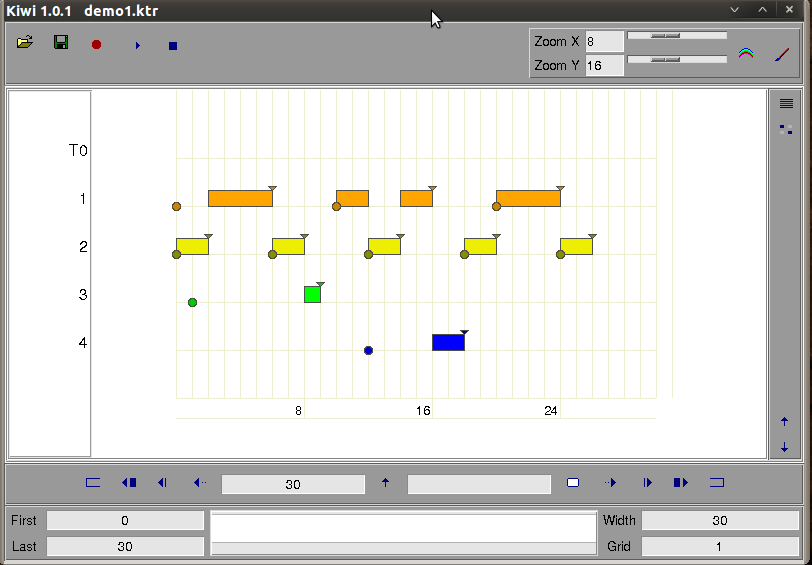
\includegraphics[scale=0.60]{img/RMBG}
  \caption{Résultat de l'appelle à RMBG}
  \label{fig:RMBG}
\end{figure}
On obtient les résultat suivants suivants : 

****BILAN ET ANALYSE****
Temps d'execution : 30
Temps creux : 5
Utilisation du processeur :83
Nombre de préemptions :1
****TacheAp****
Temps de réponse min : 4
Temps de réponse max : 7
Temps de réponse moy : 6.5
